\chapter{Prozesserstellung}

sagen dass man eine art kochrezept will

\section{Vorhandene Daten}
Ausgangsparameter test
\subsection{Wer (Akteure}
\subsection{Was (Daten)}
\subsection{Warum (Anforderungen/Usecases)}
\subsection{Womit (Komponenten)}

\section{Prozesserstellungsversuche}
Ausgehend von den vorhandenen Daten wurden mehrere Prozesse definiert, welche bis auf den Letzten entweder zu grobe Ergebnisse lieferten, oder nicht nachvollziehbar waren.

Ausgangsbasis war eine Systemvision mit folgenden Anforderungen:

\begin{itemize}
  \item Es soll eine Webseite entstehen, welche die Prüfungstermine auflistet und Personen erlaubt, sich für diese Prüfungen anzumelden
  \item Die Übermittlung der Prüfungsdaten soll über einen eigenen VPN Server geschehen
  \item Die Prüfungsdaten werden firmenintern verwaltet und nach der Auswertung soll der Scheme Owner benachrichtigt werden
\end{itemize}

\begin{figure}[!htbp]
    \centering
    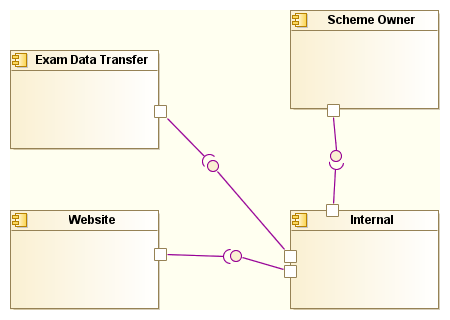
\includegraphics[scale=0.6]{uml/vision.png}
    \caption{Systemvision der Komponenten}
\end{figure}

Aufbauend darauf wurde dann versucht einen Prozess zu finden, der diese Grundideen berücksichtigt.

\subsection{Vom Usecase zur Komponente}
Der erste Versuch zur Erstellung des Architekturprozesses orientierte sich am Prinzip: teile und herrsche. Der Prozess hing stark von den nicht funktionalen Anforderungen ab und sollte auf folgender Weise funktionieren:

\begin{itemize}
  \item Für jeden Usecase wird ein komplettes Komponentendiagramm des Systems erstellt
  \item Die Komponenten jedes Teilsystems werden anhand ihrer nicht funktionalen Qualitäten aus einem Pool von Komponentenarchitekturen gewählt
  \item Schlussendlich werden alle Teilsysteme mit einander vereinigt, soweit es die nicht funktionalen Attribute erlauben
\end{itemize}

Dieser Prozess scheiterte nicht nur am enormen Modellierungsaufwand, sondern auch am Auswahlprozess der Komponenten: Je nachdem, welche Komponentenarchitekturen vorhanden waren und wie diese bewertet wurden, entstanden unterschiedliche Architekturen. Zudem schien es zu viele Komponentenarchitekturen zu geben, da die einzelnen Komponenten beliebig miteinander kombinierbar waren.

Die Qualität der Architektur hätte folglich von der Vollständigkeit dieser scheinbar unendlich großen Menge an Komponentenarchitekturen abgehangen. Aus diesem Grund schien er ungeeignet und wurde verworfen.

\subsection{Von einer geschätzten Architektur auf eine verfeinerte Architektur durch nicht funktionale Anforderungen}
Zweiter Versuch: Nach Erfahrungswerten so viel wie möglich erstellen, danach überprüfen auf nicht funktionale Anforderungen und notwenige Änderungen einbringen -> kein Kochrezept, verlässt sich zu viel auf Erfahrungswerte
\subsection{Von den Daten zur Architektur}
Dritter Versuch: Aufspalten der Architektur in Datenbereiche. Ging schon gut aber Ergebnis zu grob
\subsection{Von den Daten und den Akteuren zur Architektur}
Vierter: Einbeziehen der Akteure
